\section{Internal architecture}
The lot controller will comprises of 4 subcomponents: \textit{MainComponent, IOComponent, EmptyComponent and ProjectComponent}.

\textit{MainComponent} receives information about the lots in the tray and the need for calibration, this information is distributed to the relevant components Furthermore it makes sure that once all lots are processed that the system will go to its final state and finishes.

\textit{IOComponent} is responsible for keeping robot $r_1$ busy, it places wafers onto chuck $p_{in}$ and pre-measures them whenever possible. Also whenever a wafer is at $p_{out}$ \textit{IOComponent} will place this wafer on the tray. Information about the number of wafers to take from and to place onto the tray is communicated with the \textit{MainComponent}. \textit{ProjectComponent} and \textit{IOComponent} keep each other up to date about the status of $p_{in}$ and $p_{out}$.

\textit{ProjectComponent} is responsible for the measurement and projection of the wafers, wafers that are pre-measured and located a $p_{in}$ are moved by the \textit{ProjectComponent}, measured, projected and placed onto chuck $p_{out}$. \textit{ProjectComponent} is also responsible to calibrate whenever this is required. \textit{ProjectComponent} receives information about the recipe and about the need for calibration from \textit{MainComponent}. It interacts with \textit{IOComponent} about the statues of $p_{in}$ and $p_{out}$. Furthermore it utilizes the \textit{EmptyComponent} to place or remove closing wafers.

\textit{EmptyComponent} subordinates to \textit{ProjectComponent} and places or removes a closing wafer on/from $p_{meas}$ whenever desired by \textit{ProjectComponent}.\\

\begin{figure}
	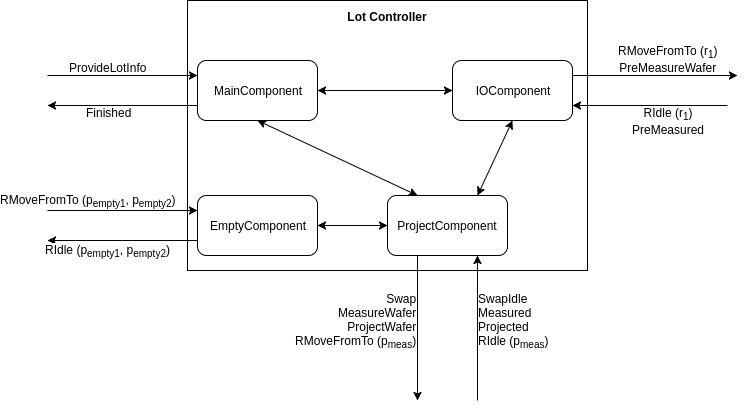
\includegraphics[width=\textwidth]{img/internal_architecture.png}
    \caption{Internal architecture}
    \label{fig:internal_arch}
\end{figure}
Figure \ref{fig:internal_arch} shows the different internal components as well as the interactions they perform with external systems. 

\subsection{Internal interactions}
Besides the external interactions the system utilizes internal interactions to communicate between the different internal components. \\
\textbf{MainComponent to IOComponent:}
	\begin{itemize}
	\item  \textit{AvailableWafers(n)}\\
	Communicates the amount of wafers that are on the current lot where $n \in \mathbb{N}$ is the amount of wafers.
	\end{itemize}
\textbf{IOComponent to MainComponent:}
	\begin{itemize}
	\item  \textit{CompletedLot}\\
	Indicates that all the wafers on the current lot are placed onto the tray.
	\end{itemize}
\textbf{MainComponent to ProjectComponent:}
	\begin{itemize}
	\item  \textit{ChangeConfig(r, c)}\\
	Communicate a change in lot configuration which includes the recipe as well as the need for calibration. $r \in Q$ is the recipe and $c \in \mathbb{B}$ indicates whether or not calibration is needed.
	\end{itemize}
\textbf{ProjectComponent to MainComponent:}
	\begin{itemize}
	\item  \textit{ChangedConfig}\\
	Indicates that the configuration has been changed.
	\end{itemize}
\textbf{IOComponent to ProjectComponent:}
	\begin{itemize}
	\item  \textit{WaferReadyAtChuckIn}\\
	Indicates that a wafer is at $p_\mathit{in}$ which has been pre-measured.
	\item  \textit{WaferTakenAtChuckOut}\\
	Indicates that the wafer that was on $p_\mathit{out}$ has been placed onto the tray.
	\end{itemize}
\textbf{ProjectComponent to IOComponent:}
	\begin{itemize}
	\item  \textit{WaferReadyAtChuckOut}\\
	Indicates that a wafer is at $p_\mathit{out}$ which has been projected.
	\item  \textit{WaferTakenAtChuckIn}\\
	Indicates that the wafer that was on $p_\mathit{in}$ has been moved to $p_\mathit{meas}$.
	\end{itemize}
\textbf{ProjectComponent to EmptyComponent:}
	\begin{itemize}
	\item  \textit{ProvideClosingWafer}\\
	Request a closing wafer to be placed at $p_\mathit{meas}$.
	\item  \textit{StoreClosingWafer}\\
	Request the closing wafer to be removed from $p_\mathit{meas}$.
	\end{itemize}
\textbf{EmptyComponent to ProjectComponent:}
	\begin{itemize}
	\item  \textit{ProvidedClosingWafer}\\
	Indicates that a closing wafer has been placed at $p_\mathit{meas}$.
	\item  \textit{StoredClosingWafer}\\
	Indicates that a closing wafer has been removed from $p_\mathit{meas}$.
	\end{itemize}